\tikzset{every picture/.style={line width=0.75pt}} %set default line width to 0.75pt        

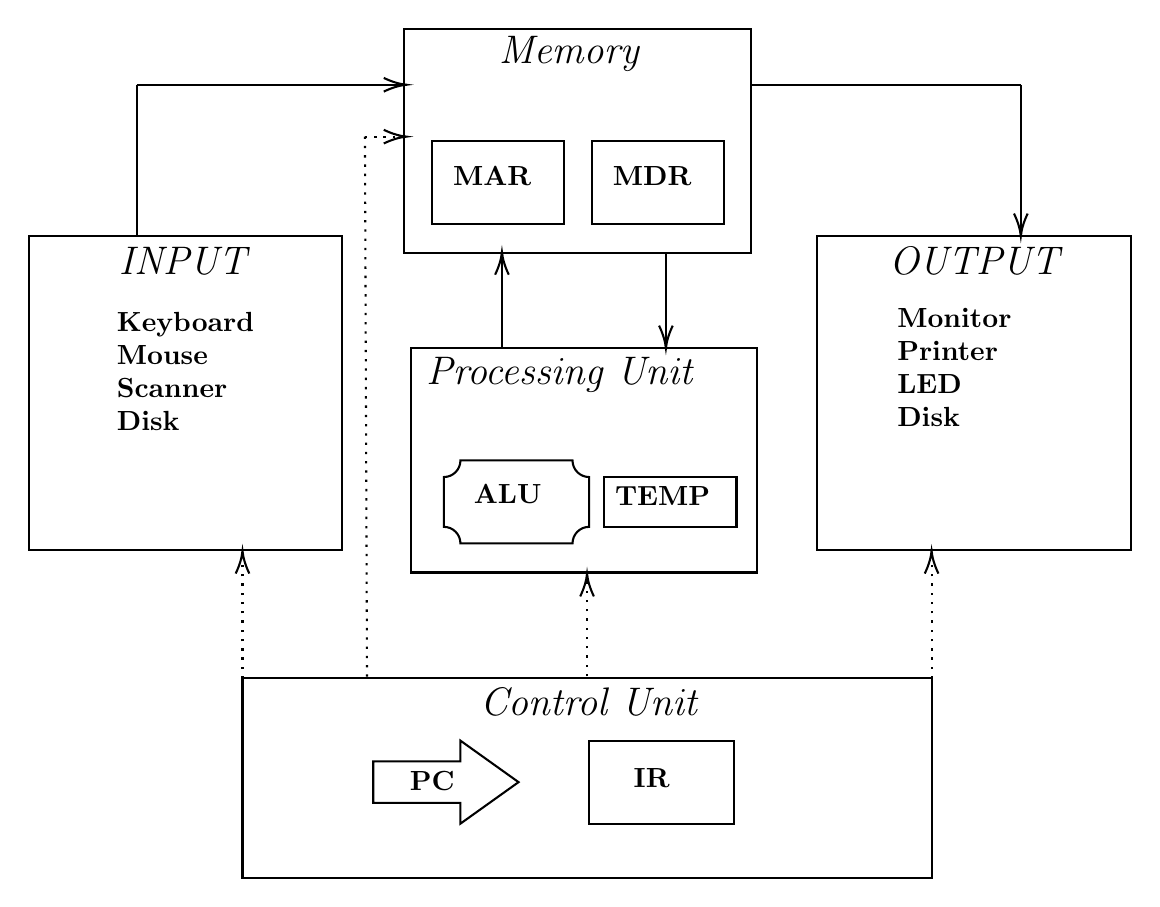
\begin{tikzpicture}[x=0.75pt,y=0.75pt,yscale=-1,xscale=1]
%uncomment if require: \path (0,536); %set diagram left start at 0, and has height of 536

%Shape: Square [id:dp6842021214778704] 
\draw   (38,107) -- (189,107) -- (189,258) -- (38,258) -- cycle ;
%Shape: Square [id:dp2846781522874837] 
\draw   (418,107) -- (569,107) -- (569,258) -- (418,258) -- cycle ;
%Shape: Rectangle [id:dp7000294601399879] 
\draw   (141,320) -- (473,320) -- (473,416) -- (141,416) -- cycle ;
%Right Arrow [id:dp27948617576185875] 
\draw   (204,360) -- (246,360) -- (246,350) -- (274,370) -- (246,390) -- (246,380) -- (204,380) -- cycle ;
%Shape: Rectangle [id:dp5238183889968957] 
\draw   (308,350) -- (378,350) -- (378,390) -- (308,390) -- cycle ;
%Shape: Rectangle [id:dp4274195934195226] 
\draw   (222,161) -- (389,161) -- (389,269) -- (222,269) -- cycle ;
%Shape: Rectangle [id:dp8158827848725543] 
\draw   (219,7) -- (386,7) -- (386,115) -- (219,115) -- cycle ;
%Shape: Rectangle [id:dp5804130759863328] 
\draw   (232.5,61) -- (296,61) -- (296,101) -- (232.5,101) -- cycle ;
%Shape: Rectangle [id:dp12227146904878561] 
\draw   (309.5,61) -- (373,61) -- (373,101) -- (309.5,101) -- cycle ;
%Shape: Plaque [id:dp995424536451063] 
\draw   (238,223) .. controls (242.42,223) and (246,219.42) .. (246,215) -- (300,215) .. controls (300,219.42) and (303.58,223) .. (308,223) -- (308,247) .. controls (303.58,247) and (300,250.58) .. (300,255) -- (246,255) .. controls (246,250.58) and (242.42,247) .. (238,247) -- cycle ;
%Shape: Rectangle [id:dp6361147141573973] 
\draw   (315,223) -- (379,223) -- (379,247) -- (315,247) -- cycle ;
%Straight Lines [id:da8084212324067266] 
\draw  [dash pattern={on 0.84pt off 2.51pt}]  (141,320) -- (141,260.58) ;
\draw [shift={(141,258.58)}, rotate = 90] [color={rgb, 255:red, 0; green, 0; blue, 0 }  ][line width=0.75]    (10.93,-3.29) .. controls (6.95,-1.4) and (3.31,-0.3) .. (0,0) .. controls (3.31,0.3) and (6.95,1.4) .. (10.93,3.29)   ;
%Straight Lines [id:da4139933874047299] 
\draw  [dash pattern={on 0.84pt off 2.51pt}]  (473,320) -- (473,260.58) ;
\draw [shift={(473,258.58)}, rotate = 90] [color={rgb, 255:red, 0; green, 0; blue, 0 }  ][line width=0.75]    (10.93,-3.29) .. controls (6.95,-1.4) and (3.31,-0.3) .. (0,0) .. controls (3.31,0.3) and (6.95,1.4) .. (10.93,3.29)   ;
%Straight Lines [id:da6375241441773398] 
\draw  [dash pattern={on 0.84pt off 2.51pt}]  (307,319) -- (307,271.58) ;
\draw [shift={(307,269.58)}, rotate = 90] [color={rgb, 255:red, 0; green, 0; blue, 0 }  ][line width=0.75]    (10.93,-3.29) .. controls (6.95,-1.4) and (3.31,-0.3) .. (0,0) .. controls (3.31,0.3) and (6.95,1.4) .. (10.93,3.29)   ;
%Straight Lines [id:da7823928920015608] 
\draw  [dash pattern={on 0.84pt off 2.51pt}]  (200,59) -- (201,320) ;
%Straight Lines [id:da0832406275103772] 
\draw  [dash pattern={on 0.84pt off 2.51pt}]  (200,59) -- (218,59) ;
\draw [shift={(220,59)}, rotate = 180] [color={rgb, 255:red, 0; green, 0; blue, 0 }  ][line width=0.75]    (10.93,-3.29) .. controls (6.95,-1.4) and (3.31,-0.3) .. (0,0) .. controls (3.31,0.3) and (6.95,1.4) .. (10.93,3.29)   ;
%Straight Lines [id:da6550156642776477] 
\draw    (266,161) -- (266,116.58) ;
\draw [shift={(266,114.58)}, rotate = 90] [color={rgb, 255:red, 0; green, 0; blue, 0 }  ][line width=0.75]    (10.93,-3.29) .. controls (6.95,-1.4) and (3.31,-0.3) .. (0,0) .. controls (3.31,0.3) and (6.95,1.4) .. (10.93,3.29)   ;
%Shape: Boxed Line [id:dp25364397431402463] 
\draw    (345,114.58) -- (345,159) ;
\draw [shift={(345,161)}, rotate = 270] [color={rgb, 255:red, 0; green, 0; blue, 0 }  ][line width=0.75]    (10.93,-3.29) .. controls (6.95,-1.4) and (3.31,-0.3) .. (0,0) .. controls (3.31,0.3) and (6.95,1.4) .. (10.93,3.29)   ;
%Straight Lines [id:da5907462027159831] 
\draw    (90,34) -- (90,107) ;
%Straight Lines [id:da14006758297346078] 
\draw    (90,34) -- (218,34) ;
\draw [shift={(220,34)}, rotate = 180] [color={rgb, 255:red, 0; green, 0; blue, 0 }  ][line width=0.75]    (10.93,-3.29) .. controls (6.95,-1.4) and (3.31,-0.3) .. (0,0) .. controls (3.31,0.3) and (6.95,1.4) .. (10.93,3.29)   ;
%Straight Lines [id:da5528848956046384] 
\draw    (516,34) -- (516,105) ;
\draw [shift={(516,107)}, rotate = 270] [color={rgb, 255:red, 0; green, 0; blue, 0 }  ][line width=0.75]    (10.93,-3.29) .. controls (6.95,-1.4) and (3.31,-0.3) .. (0,0) .. controls (3.31,0.3) and (6.95,1.4) .. (10.93,3.29)   ;
%Straight Lines [id:da4578186118418053] 
\draw    (516,34) -- (386,34) ;

% Text Node
\draw (80,111) node [anchor=north west][inner sep=0.75pt]   [align=left] {\textit{{\Large INPUT}}};
% Text Node
\draw (79,142) node [anchor=north west][inner sep=0.75pt]   [align=left] {\textbf{Keyboard}\\\textbf{Mouse}\\\textbf{Scanner}\\\textbf{Disk}};
% Text Node
\draw (451,111) node [anchor=north west][inner sep=0.75pt]   [align=left] {\textit{{\Large OUTPUT}}};
% Text Node
\draw (455,140) node [anchor=north west][inner sep=0.75pt]   [align=left] {\textbf{Monitor}\\\textbf{Printer}\\\textbf{LED}\\\textbf{Disk}};
% Text Node
\draw (254,323) node [anchor=north west][inner sep=0.75pt]   [align=left] {\textit{{\Large Control Unit}}};
% Text Node
\draw (232.42,369.5) node   [align=left] {\textbf{PC}};
% Text Node
\draw (328,362) node [anchor=north west][inner sep=0.75pt]   [align=left] {\textbf{IR}};
% Text Node
\draw (228,164) node [anchor=north west][inner sep=0.75pt]   [align=left] {{\Large \textit{Processing Unit}}};
% Text Node
\draw (263,9) node [anchor=north west][inner sep=0.75pt]   [align=left] {{\Large \textit{Memory}}};
% Text Node
\draw (241,72) node [anchor=north west][inner sep=0.75pt]   [align=left] {\textbf{MAR}};
% Text Node
\draw (318,72) node [anchor=north west][inner sep=0.75pt]   [align=left] {\textbf{MDR}};
% Text Node
\draw (251,225) node [anchor=north west][inner sep=0.75pt]   [align=left] {\textbf{ALU}};
% Text Node
\draw (319,226) node [anchor=north west][inner sep=0.75pt]   [align=left] {\textbf{TEMP}};


\end{tikzpicture}
